% This is lnicst.tex the demonstration file of the LaTeX macro package for
% Lecture Notes of the Institute for Computer Sciences, Social-Informatics 
% and Telecommunications Engineering series from Springer-Verlag.
% It serves as a template for authors as well.
% version 1.0 for LaTeX2e
%
\documentclass[lnicst]{svmultln}
%
\usepackage{graphicx} % includegraphics
\usepackage{makeidx}  % allows for indexgeneration
\usepackage{url} %for url citing
\usepackage{caption}
\usepackage[table]{xcolor}
\usepackage{listings}
\newcommand{\F}{Fig.}

\newcommand\DejaVuttfamily{%
  \fontfamily{DejaVuSansMono-TLF}\selectfont
}
\newcommand{\eg}{\textit{e}.\textit{g}.}
\lstset{
  language=C,numbers=left,xleftmargin=2.5em,
  basicstyle=\DejaVuttfamily\scriptsize,
  keywordstyle=\color{blue}\DejaVuttfamily,
  stringstyle=\color{red}\DejaVuttfamily,
  commentstyle=\color{Bittersweet}\DejaVuttfamily,
  moredelim=**[is][\color{red}]{@}{@},
  escapeinside={<@}{@>}
}
\usepackage{amsmath}
\usepackage{algorithm}
\usepackage[noend]{algpseudocode}

% \makeindex          % be prepared for an author index
%
\begin{document}
%
\mainmatter              % start of the contribution
%
\title{Obfuscation with Turing Machine}
%
\titlerunning{Turing Obfuscation}  % abbreviated title (for running head)
%                                     also used for the TOC unless
%                                     \toctitle is used
%
\author{Yan Wang \and Shuai Wang \and Pei Wang \and Dinghao Wu}
%
%\authorrunning{Wang et al.}   % abbreviated author list (for running head)
%
%%%% list of authors for the TOC (use if author list has to be modified)
\tocauthor{Yan Wang, Shuai Wang, Pei Wang, Dinghao Wu}
%
\institute{The Pennsylvania State University\\University Park, PA 16802, USA\\
\email{{ybw5084,szw175,pxw172,dwu}@ist.psu.edu} %\\ WWW home page:
%\texttt{http://users/\homedir iekeland/web/welcome.html}
% \and
% Universit\'{e} de Paris-Sud,
% Laboratoire d'Analyse Num\'{e}rique, B\^{a}timent 425,\\
% F-91405 Orsay Cedex, France}
}
\maketitle              
% typeset the title of the contribution
% \index{Ekeland, Ivar} % entries for the author index
% \index{Temam, Roger}  % of the whole volume
% \index{Dean, Jeffrey}

\begin{abstract} % give a summary of your paper
Obfuscation is an important technique to protect software from adversary
analysis. Control flow obfuscation effectively prevents attackers from
understanding the program structure, hence impeding a broad set of reverse
engineering activities. In this paper, we propose a novel control flow
obfuscation method which employs Turing machines to simulate the computation of
branch conditions. By weaving the original program with Turing machine
components, program control flow graph and call graph would become more complex.
Moreover, due to the computation complexity of a Turing machine, program
execution flow would become much more complicated and resilient to advanced
reverse engineering approaches through symbolic execution and concolic testing.
%
We implement an prototype tool based on the proposed technique. Comparing with
previous work, our control flow obfuscation technique bears three distinct
advantages. 1). Complexity: the complicated implementation of a Turing machine
makes it hard for attackers to understand the program control flow structure.
2). Universality: theoretically, Turing machines can encode any computation. Our
obfuscation is built on top of the LLVM intermediate representation so the
application scope is broadened to almost every language with an LLVM front-end
compiler. 3). Resiliency: our obfuscation is shown to be very resilient to
advanced analysis tools. We evaluate our method in terms of functionality
correctness, potency, resilience, stealth, and cost, respectively. The
experimental results show that the proposed technique can obfuscate programs in
stealth with good performance and robustness.
\end{abstract}

\keywords {Software Security, Control Flow Obfuscation, Turing Machine}

\section{Introduction}
\label{sec:introduction}
Obfuscation is an important technique for intellectual property protection. The
Internet brings us unprecedented convenience along with idea plagiarism threat
and copyright infringement. Attackers could take advantage of the
state-of-the-art techniques~\cite{Loop,Lee,Molnar} to recover program source
code from executable files, exploit software vulnerabilities and steal algorithm
implementations. Software obfuscation is mostly designed to impede such
(malicious) reverse engineering process.

Recently, software security research again draws people's attention because of
infamous ransomware attack and severe vulnerabilities such as the ``Wannacry''
incidence and the OpenSSL ``Heartbleed'' bug~\cite{Heartbleed,wannacry}. All of
these malwares exploit vulnerabilities inside a program. To launch such attack,
attackers usually need to recover the control flow structure of the victim
programs first. Symbolic execution and concolic testing are well-developed and
widely-adopted techniques to cover execution paths and explore program
structure~\cite{dart,exe,Sen,symbol}. Typical concolic testing engines such as
SAGE~\cite{Sage} and KLEE~\cite{klee} could yield new input which leads to a new
execution path by solving branch conditions as constraints with a constraint
solver. Such tools have been proved as very effective in analyzing program
control flow structures~\cite{Cute}.

Hence, a lot of anti-reverse engineering research has focused on preventing
adversaries from analyzing important path conditions in a
program~\cite{Opaque,Sharif,Popov,Zhi, Wang:Zhi}. Control flow obfuscation is
one of these cutting-edge techniques to combat these reverse engineering tools.
Control flow obfuscation aims at hiding path conditions and complicating the
execution flow within a program. By rewriting or adding extra control flow
components, the program path conditions become difficult or even impossible to
analyze. Existing research~\cite{Ma} have demonstrated the effectiveness of
control flow obfuscation.

% \begin{figure}
%   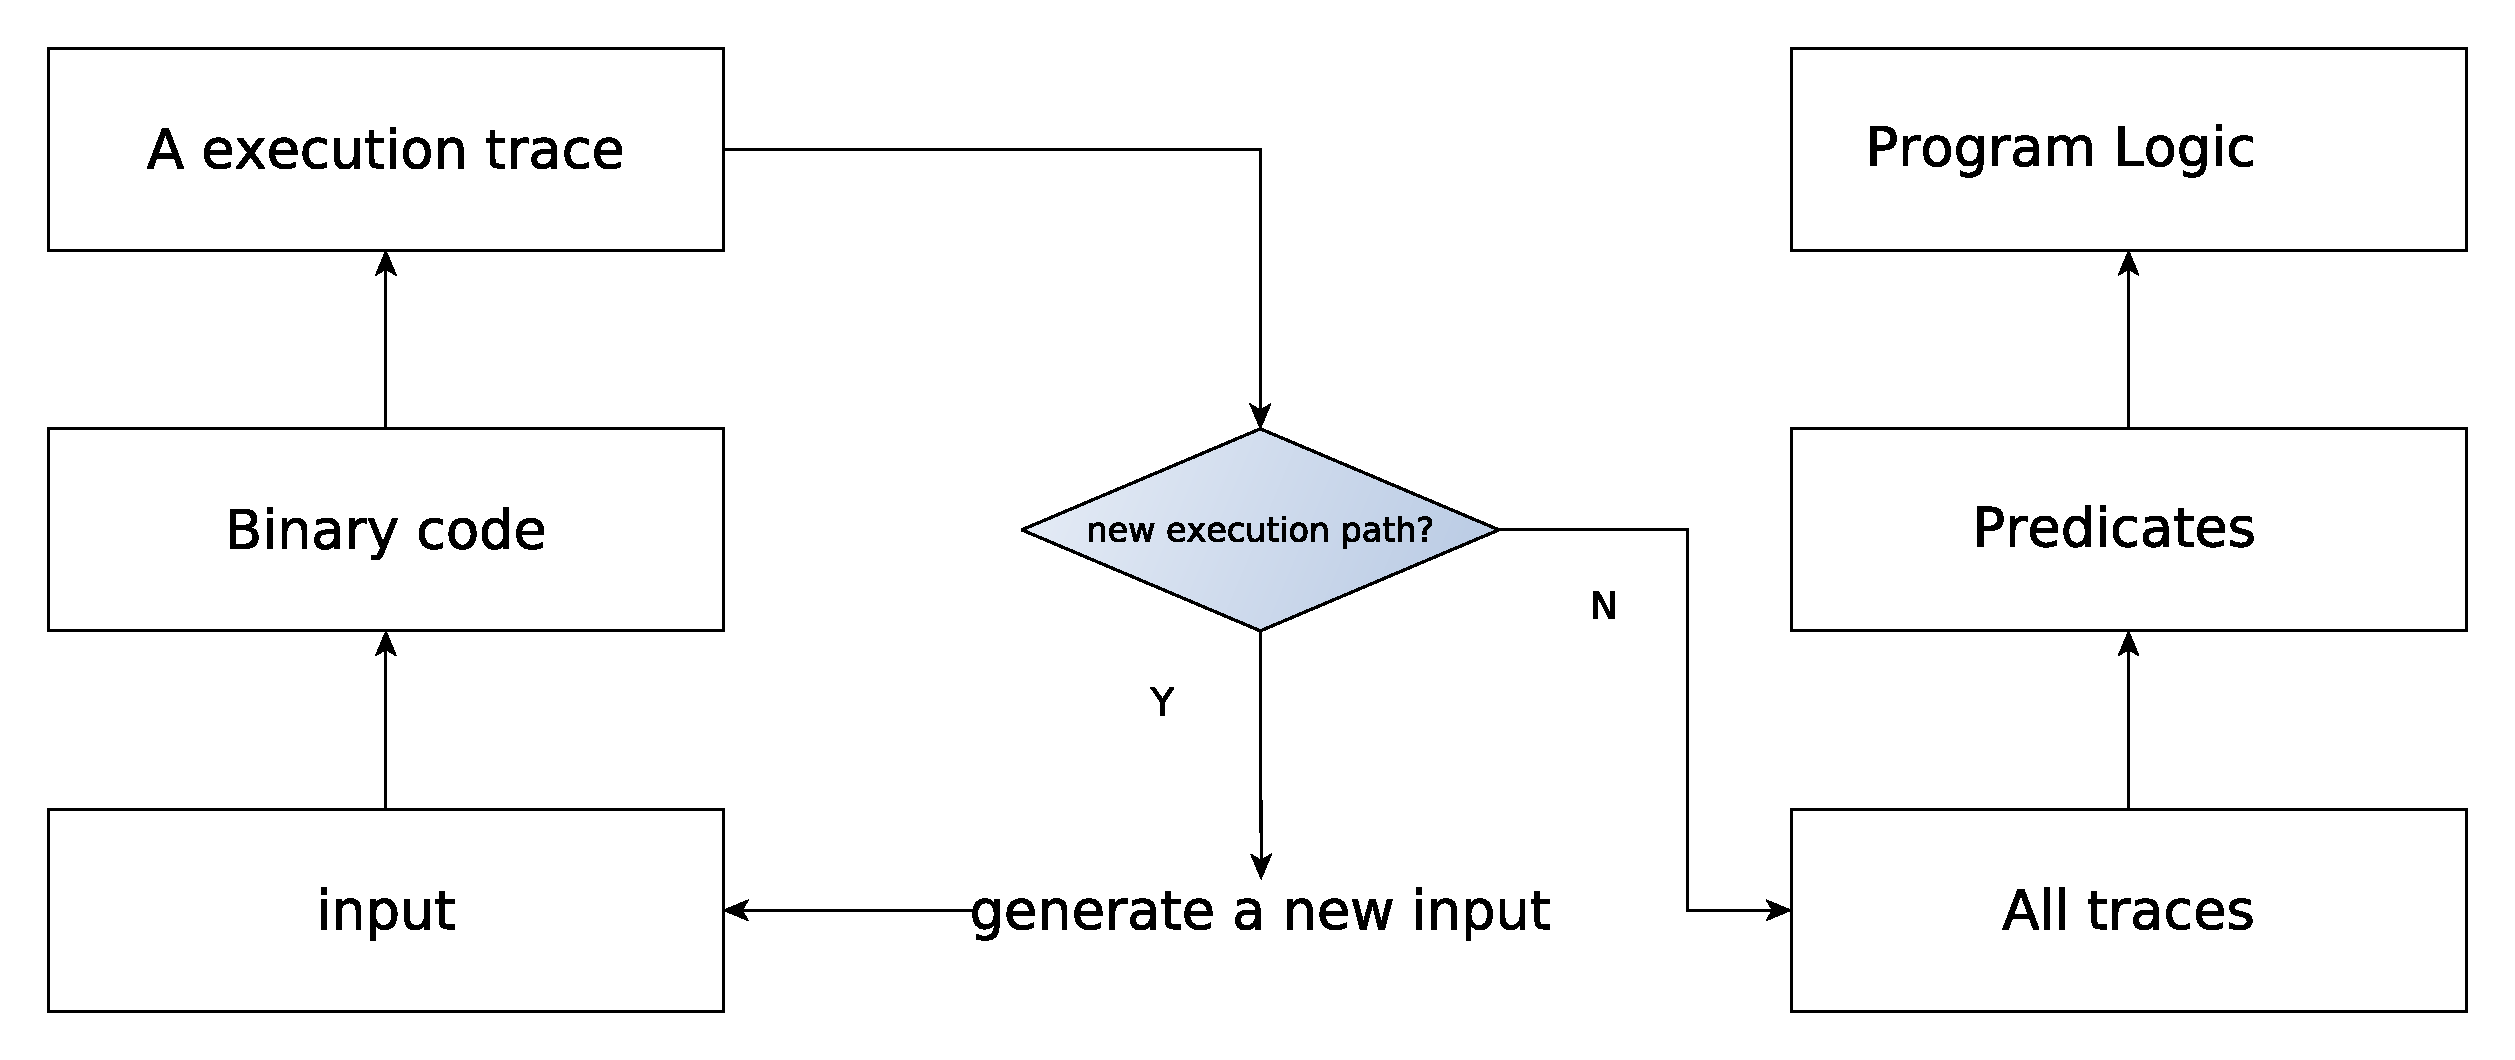
\includegraphics[width=0.9\linewidth]{reverse_engineering.eps}
%   \caption{Reverse engineering with concolic testing}
%   \label{fig:one}
% \end{figure}

In this paper, we propose a novel control flow obfuscation method which
leverages Turing machine to compute path conditions. The \textit{Church-Turing
  thesis}~\cite{Church} states that the power of Turing machines and
$\lambda$-calculus is the same as algorithms, or the informal notion of
effectively calculable functions. Formally, Turing computable,
$\lambda$-computable, and general recursive functions are shown to be
equivalent, and informally, the thesis states that they all capture the power of
algorithms or effectively calculable functions. This means any functional
component of software can be re-implemented as or transformed into a Turing
machine; the replaced code component and its corresponding semantic equivalent
Turing machine is called \textit{Turing Equivalent}.

In this work, we propose to simulate important branch condition statements in a
program with its \textit{Turing Equivalent} Turing machine. A Turing machine
behaves as a state machine so it would bring in a large amount of extra control
flow transfers and basic blocks to the overall program control flow graph.
Moreover, a typical Turing machine leverages a transition table to guide the
computation, and such transition table-based execution would introduce
additional computations and make the overall execution flow much more
complicated. We envision the proposed technique would largely complicate the
protected program, and also bring in new challenges for reverse engineering
tasks.

To obfuscate a program through the proposed Turing machine obfuscation
technique, we first translate the original program source code into a compiler
intermediate representation. Our Turing machine obfuscator then selects branch
condition statements for transformation; the transformed instructions will invoke its
corresponding Turing machine component, which is semantically equivalent to the
original branch condition. After finishing the execution in the Turing machine
``black box'', the execution flow returns back to the original instruction, with
a return value which determines the branch selection. Inspired by previous
work~\cite{Collberg}, we evaluate our obfuscator regarding five aspects which
are functionality correctness, potency, resilience, cost and stealth. Results
indicate that Turing machine obfuscator could effectively obfuscate
commonly-used software with acceptable cost and robustness.

This paper is organized as follows. Section 2 discusses related works on
obfuscation, especially control flow obfuscation. Section 3 presents the overall
design of Turing machine obfuscator. Obfuscator implementation is discussed in
Section 4. Section 5 presents the evaluation result of our proposed technique.
We further present discussion in Section 6, and conclude the paper in Section 7.

%
\section{Related Work}
Generally speaking, reverse engineering techniques are categorized into static
track and dynamic track. To battle static reverse engineering, researchers
usually focus on hardening disassembling and decompiling process. To combat the
dynamic reverse engineering techniques such as concolic testing, sensitive
conditional transfer logic must be hidden from adversaries. Control flow
obfuscation has been proved effective in this scenario.

Sharif et al.~\cite{Sharif} propose a technique to rewrite certain branch
conditions and encrypt code components that are guarded by such conditions.
Branch conditions that are dependent on the input are selected and branch
condition outputs are transformed with a hash function. Moreover, the code
component which is dependent on a transformed condition would be encrypted; the
encryption key is derived from the input which satisfies the branch condition.
In general, their technique focus on selectively translate branch conditions
that are dependent on the input, which could leave many branch conditions
unprotected. Also, since the branch condition statement itself is mostly
untouched (only the boolean output is hashed), the original branch condition
code is still in the obfuscated program, which could be leveraged to reveal the
original semantics.

Popov et al.~\cite{Popov} propose to replace unconditional control transfer
instructions such as \texttt{jmp} and \texttt{call} with ``signals''. Their work
is used to impede binary disassembly, usually the starting point of reverse
engineering. Moreover, dummy control transfers and junk instructions are also
inserted after the replaced control transfers. This method is effective in
fooling disassemblers in analyzing unconditional transfers but it becomes
mal-functional where the conditional transfers need to be protected as well.
Another related work proposes to protect control flow branches leveraging a
remote trusted third party environment~\cite{Zhi}. In general, their technique
mostly introduces notable network overhead and also relies on trusted network
accessibility which may not be feasible in practice.

Ma et al.~\cite{Ma, Maieee} propose to use neural network to replace certain
branch condition statements; the propose technique is evaluated to conceal
conditional instructions and impede typical reverse engineering analysis such as
concolic testing. Although the idea is promising and the experimental results
indicate the effectiveness to certain degree, in general neural network-based
approach may not be suitable for security applications. To the best of our
knowledge, neural network works like a black box; it lacks a rigorous
theoretical foundation to show a correct result can always to generated given an
input. In other words, neural networks may yield results which lead to an
incorrect branch selection. Overall, neural networks introduce complexity as
well as (unwanted) uncertainty to the transformed programs. In addition, we
notice that neural network usually consumes too much memory in transforming
non-trivial programs.

%
\section{Turing machine obfuscator}
%
\subsection{Design Overview}
In a program, a branch condition statement compares two operands and selects a
branch for control transfer based on the comparison result. As aforementioned,
Turing machine has been proved to be able to simulate the semantics of any
functional component of a program. Hence, any program branch condition statement
can be modeled by a Turing machine. Taking advantage of its powerful computation
ability as well as execution complexity, we propose to employ Turing machine to
obfuscate branch condition statements (the branch condition statement is
referred as ``branch predicate'' later in this paper since its output is usually
a boolean value) in a program. A Turing machine obfuscated branch condition
statement is shown in \F~\ref{fig:two}. Instead of directly computing a boolean
value through a comparison instruction, we feed a Turing machine with the inputs
(the value of operands) and let the Turing machine to simulate the comparison
semantics.

\begin{figure}
 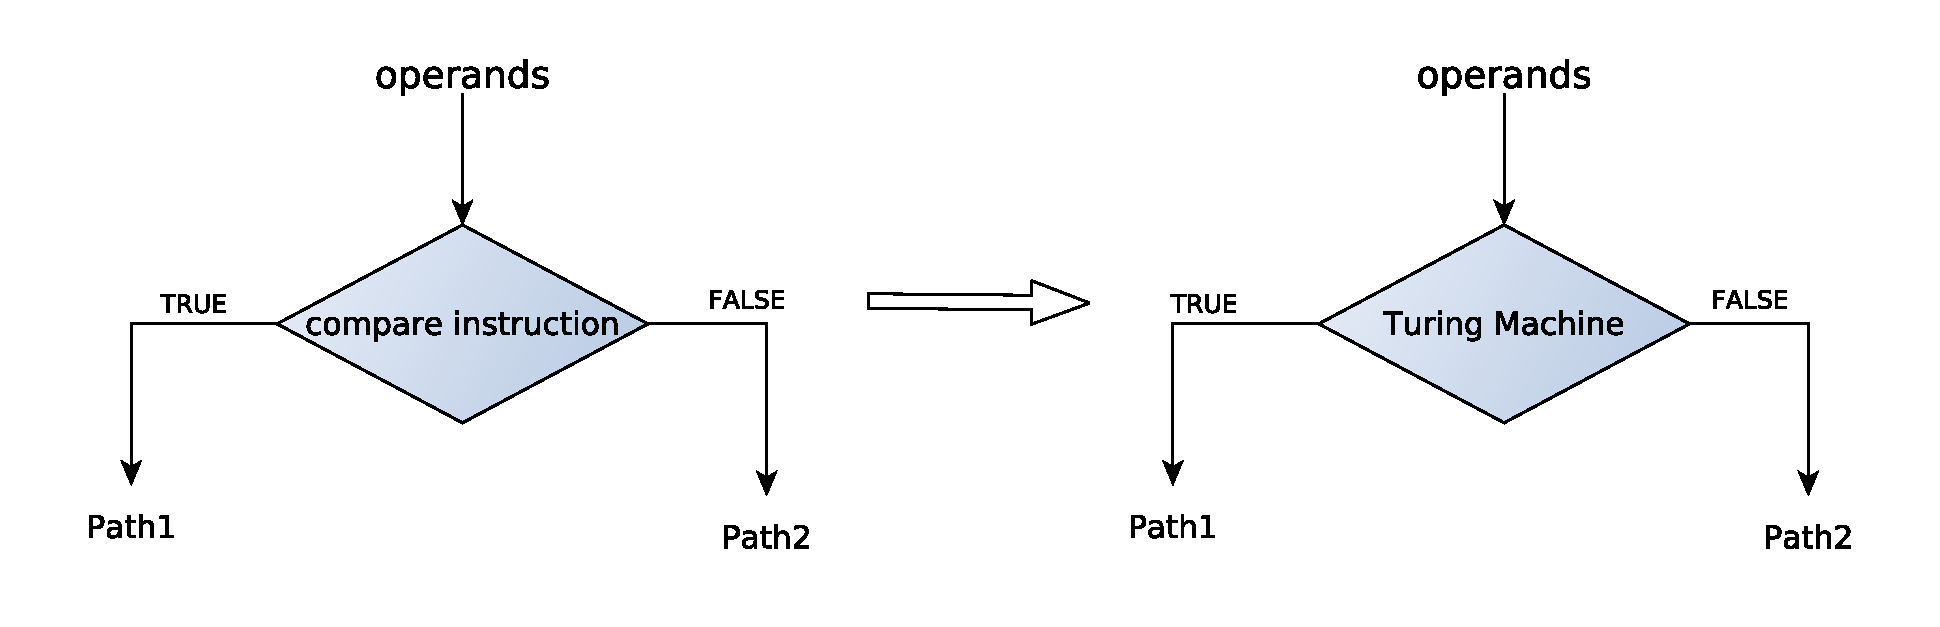
\includegraphics[width=\linewidth]{figure2.eps}
 \caption{Obfuscate a branch condition statement through a Turing machine.}
 \label{fig:two}
\end{figure}

\subsection{Turing Machine}
As shown in \F~\ref{fig:three}, a typical Turing machine consists of four
components:
\begin{itemize}
  \item An infinite-long tape which contains a sequence of cells. Each cell
    holds a symbol defined in the tape alphabet (the alphabet is introduced
    shortly). In this work, our proposed Turing machine obfuscator would
    dynamically allocate new tape cells to construct an infinite tape to store
    intermediate results.
  \item A tape head which could perform \texttt{read}, \texttt{write},
    \texttt{move left} and \texttt{move right} operations over the tape.
  \item A state register used to record the state of the Turing machine. Turing
    machine states are finite and defined in the transition table.
  \item A transition table that consists of all the transition rules defining
    how a Turing machine transfers from one state to another.
\end{itemize}

Although simple, Turing machine model resembles a modern computer in several
ways. The head is I/O device. The infinite tape acts as the computer memory. The
transition table defines the mission of this Turing machine which is like the
program code and data. Hence, Turing machine is also deemed as the foundation of
modern computer science development.

\begin{figure}
 \includegraphics[width=0.9\linewidth]{TM.pdf}
 \caption{Turing machine components.}
 \label{fig:three}
\end{figure}

\subsubsection{Transition Table}
A transition rule could be represented by a five-element tuple $(S_c, T_c, S_n,
T_n, D)$ where:

\begin{itemize}
  \item \(S_c\) is the current Turing machine state
  \item \(T_c\) is the current tape cell symbol read by the head
  \item \(S_n\) is the new Turing machine state
  \item \(T_n\) is the symbol head writes to the current tape cell
  \item \(D\) is the direction the head should move (i.e., ``left'' or
    ``right'')
\end{itemize}

In general, every five-element tuple represents a transition table rule shown in
\F~\ref{fig:three}.

\subsubsection{Turing Machine Encoding}
Initially, Turing machine is at the ``start'' (\(S_0\)) state and tape records
the Turing machine input. Consistent with existing Turing machine simulator
project~\cite{SingleTape}, blank symbol is denoted as ``*'' on the tape, while
the length of ``$\cdot$'' is used to encode an operand of integer type (our
current implementation only focuses on operand of integer type, we present
further discussion on this in \S\ref{subsec:phase-three}). For instance, integer
5 is represented as five continuous ``$\cdot$'' on the tape. Note that a Turing
machine could be encoded with various of ways, our prototype represents only one
of them. Turing machine with different encoding strategies operates with totally
distinct execution pattern. This also makes Turing machine obfuscation hard to
be analyzed.

In general, our Turing machine tape alphabet includes two symbols, i.e.,
$\{\cdot,*\}$. The tape in \F~\ref{fig:three} shows an initial state of a Turing
machine. The head of Turing machine is placed on the leftmost cell. Different
integer operands are separated by a blank symbol ``*''. Operands encoded on
the tape of \F~\ref{fig:three} are five and one. When Turing machine starts to
run, the head reads the current tape cell, combines with current state register
to locate a transition rule in the transition table, and then moves to next
state accordingly.

\subsubsection{Turing Machine Execution}
The Turing machine keeps running step by step directed by the transition table
until it reaches a \texttt{Halt} state. On the other hand, Turing machine may
keep running forever since the process of solving some problems cannot
terminate. In our research, we implement a Turing machine to simulate branch
predicates (i.e., simple algebra computations) so it should always reach a
\texttt{Halt} state. When reaching the \texttt{Halt} state, the machine stops
running and the computation result is shown on the tape. Table~\ref{table:1}
shows a transition table example, which supports a Turing machine to conduct the
addition operation in our implementation.

\begin{table}
\centering
\begin{tabular}{ |c|c|c|c|c|} 
  \hline
  \textbf{Current State} & \textbf{Current Symbol} & \textbf{New State} & \textbf{New Symbol} & \textbf{Direction} \\ 
  \hline
  \(S_0\) & * & \(S_0\) & * & Right\\ 
  \hline
  \(S_0\) & . &\(S_1\)  & . & Right\\
  \hline
  \(S_1\) & * &\(S_2\) & . & Right\\  
  \hline
  \(S_1\) & . & \(S_1\) & . & Right \\
  \hline
  \(S_2\) & * & \(S_3\) & * & Left \\
  \hline
  \(S_2\) & . & \(S_2\) & . & Right \\
  \hline
  \(S_3\) & * & \(S_3\) & * & Left \\
  \hline
  \(S_3\) & . & \(S_4\) & * & Left \\
  \hline
  \(S_4\) & * & \(Halt\) & * & - \\
  \hline
  \(S_4\) & . & \(S_4\) & . & Left\\
  \hline

\end{tabular}
\caption{Transition table of the \texttt{add} operation in a Turing machine.}
\label{table:1}
\end{table}

\subsubsection{Addition Turing Machine}
In this section, we elaborate the design of the addition Turing machine which
simulates the semantics of the \texttt{add} operation. Other Turing machines
(e.g., subtraction and multiplication Turing machine) used in this research are
designed in a similar way. Through constructing this machine, we essentially
build rules which could concatenate two series of  $\cdot$ cells on the tape
together. Take initial tape in \F~\ref{fig:three} as an example. Following the
rules in table \ref{table:1}, after a sequence of read and write operations
based on the transition table, left operand (integer value 5) and right operand
(integer value 1) which are separated by a blank symbol ``*'' are merged into a
long series of $\cdot$ cells on tape; the length of the outcome dot cells is 6,
which represents integer value 6 as shown in \F~\ref{fig:turing_outcome}.

\begin{figure}
 \includegraphics[width=0.9\linewidth]{Turingaddoutcome.pdf}
 \caption{Turing machine execution result.}
 \label{fig:turing_outcome}
\end{figure}

Reading transition table directly is difficult for a human being. To represent a
understandable description on how the transition table for the addition
operation works, we summarize the transition table logic and represent it in an
algorithm description. Algorithm~\ref{adding} describes the transition table; in
fact it states a method to combine two sequences of dot cells on tape into a
longer sequence of cells. Following the algorithm, the isolator cell (i.e., the
blank symbol) is written to $\cdot$ when Turing machine finally enter the ``Halt'' state.

\begin{algorithm}
\caption{Description of the addition transition table.}
\label{adding}
\begin{algorithmic}[1]
\Procedure{}{}
\State $\textit{head} \gets \text{the blank cell before the left operand starting cell}$
\While{$\text{head}$ != the blank cell after the right operand}
 move right\;
\EndWhile

\State move left
\State $\text{the last dot cell of the right operand} \gets \text{blank symbol}$

\While{$\text{head}$ != the blank cell within these two operands}{
  move left\;
}
\EndWhile
\State $\text{the blank cell} \gets \text{dot}$
\While{$\text{head}$ != the blank cell before the left operand}
  move left\;
\EndWhile
\State \textbf{Halt;}
\EndProcedure
\end{algorithmic}
\end{algorithm}

\subsubsection{Turing Machine of Other Operations}
%As previously discussed, given any program algorithm, there must exist a
%corresponding Turing machine. 
Since our Turing machine obfuscator essentially
focuses on obfuscating branch predicates which usually involve with arithmetic operations, Turing machine obfuscator also needs to
provide other transition tables of arithmetic operations (such as $ -, \times,
\div$).

To implement the arithmetic operations, besides the addition transition table
shown in Table~\ref{table:1}, we construct three more transition tables for subtraction,
multiplication and division operations. Their transition tables are relatively
more complex than Table~\ref{table:1}. Actually in our implementation, we build
transition table consisting of 16, 34 and 80 transition rules entries for
subtraction, multiplication and division Turing machines, respectively. As for
the comparison operations such as \(\leq, \geq, \neq\), we take advantage of the
subtraction Turing machine to calculate them. Based on the calculation result, a
boolean value is returned. In sum, we construct 4 transition tables, with
overall 140 transition table entries.

\subsection{Universal Turing Machine}
While a Turing machine could perform powerful algorithm simulation, its
computation ability is predetermined by its initial tape state and intrinsic
transition table. For instance, a Turing machine capable of doing addition
operation could only simulate the ``add'' operation since other operations would
have very different transition rules. That is, an ``add'' Turing machine could
not represent the ``subtract'' operations. Also, since the initial state needs
to be encoded on the tape before the computation, a Turing machine encoded with
$2 + 3$ could not conduct addition operation for $5 + 6$.

In non-trivial programs, branch predicate could include various arithmetic and
comparison operations, and many of these expressions would correspond to
different Turing machines. Hence, we need an unified translator to represent
arbitrary computations. Universal Turing machine is designed to simulate
arbitrary computations. As shown in \F~\ref{fig:four}, both input data and
transition table are initialized on tape as a single tape universal Turing machine. 
In some sense, a universal Turing machine acts as the
interface for us to employ Turing machines of different semantics.

Universal Turing machine bears the essence of the modern computer which is being
programmable. Through storing different transition tables and inputs on the tape
(we discuss how to construct such tapes in our research shortly), an universal
Turing machine can actually perform semantic equivalent computation to arbitrary
programs; as aforementioned, such Universal Turing Machine and the replaced
expression are \textit{Turing Equivalent}. In our Turing machine obfuscator,
different branch predicates invoke a unified interface, which bridges the
obfuscated instruction and a universal Turing machine.

\begin{figure}
 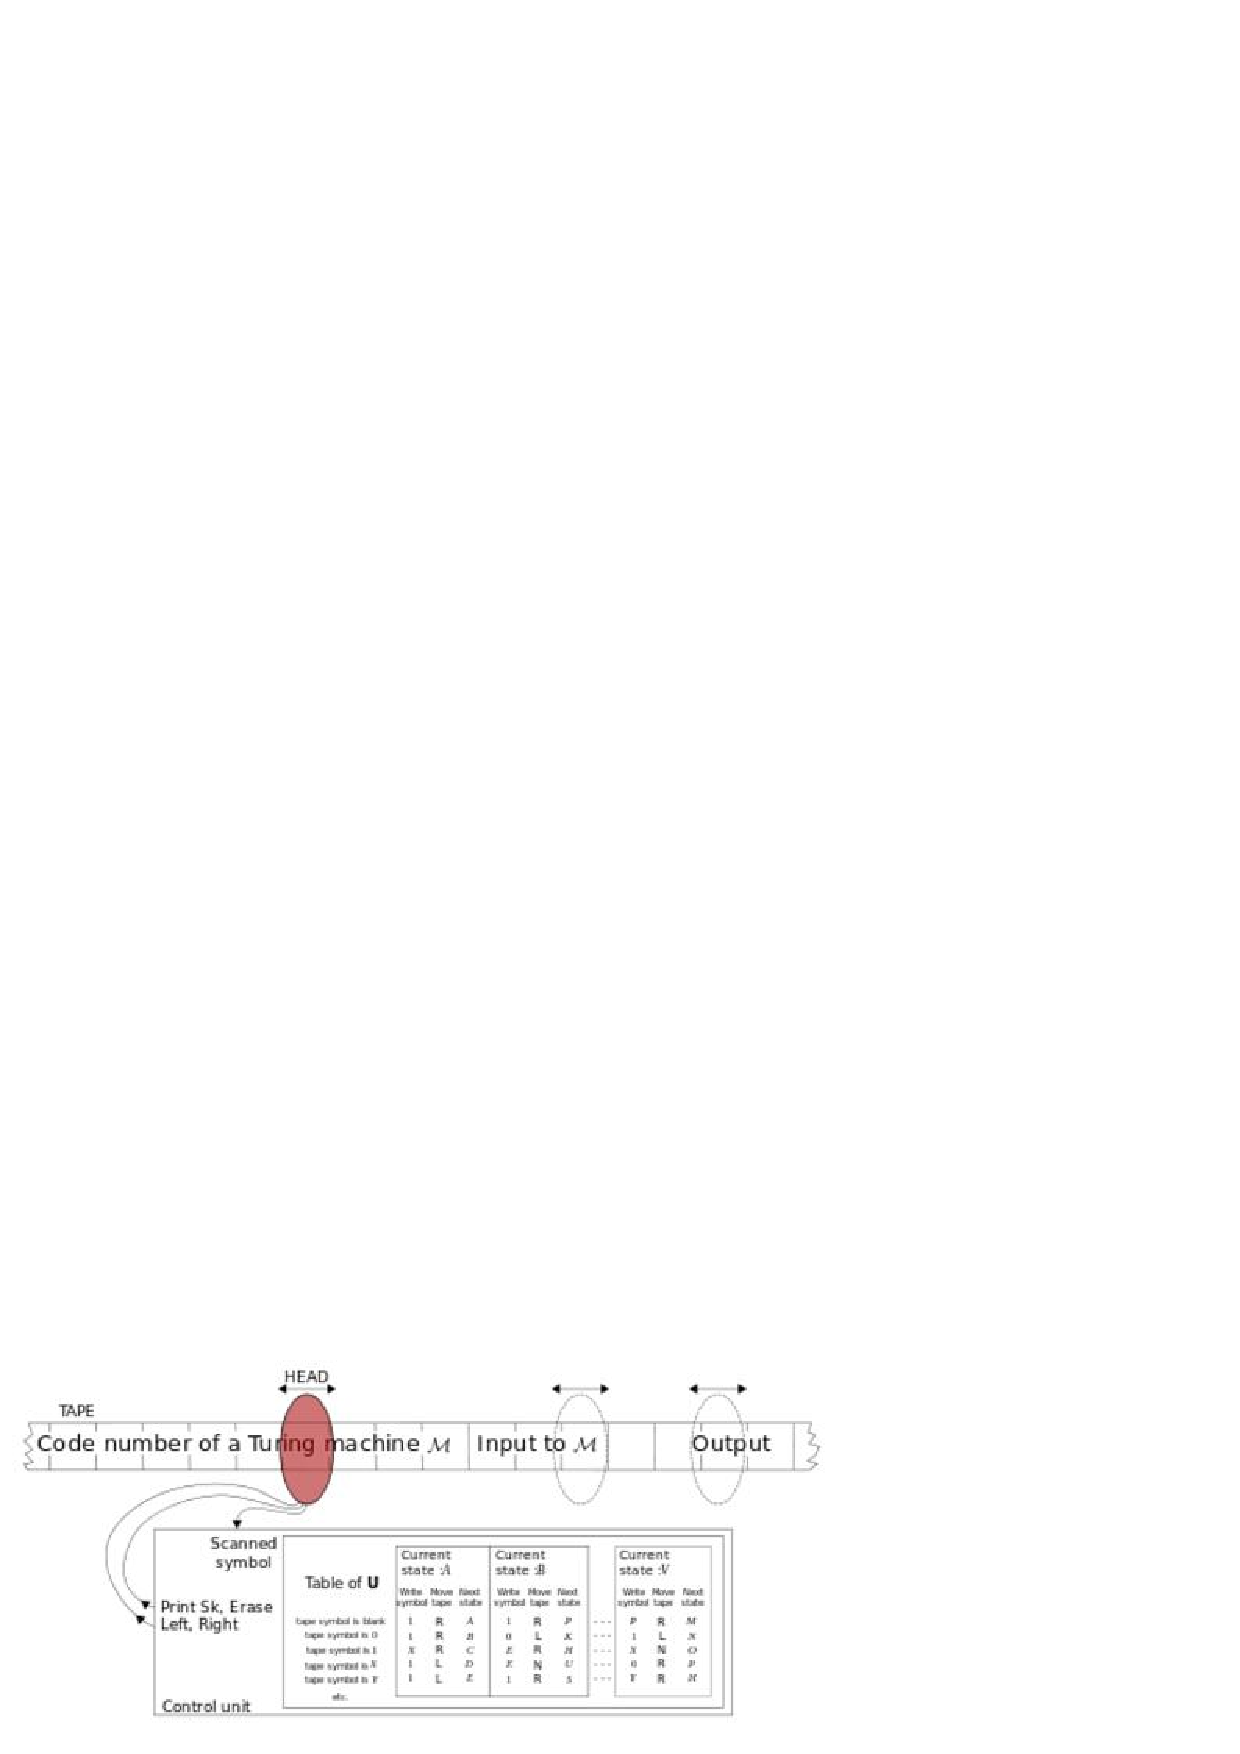
\includegraphics[width=\linewidth]{UTM.pdf}
 \caption{Universal Turing machine.}
 \label{fig:four}
\end{figure}

\subsubsection{Tape Construction}
To build the tape for a Turing machine, the universal Turing machine needs to
store all the transition tables. In this way, all the information needed for
computations exists. Later, for an incoming computation, we create a new tape,
encode the input onto the tape and select a proper transition table.
High-levelly, a ``switch'' statement over the incoming computation type is used
to select a proper transition table at this step.

\section{Implementation}
Our proposed obfuscator is made up of several components including an universal
Turing machine model implemented in C and several transformation passes based on
the LLVM compiler suite~\cite{LLVM}; As shown in \F~\ref{fig:five}, our Turing
obfuscator performs a three-phase process to generate the obfuscated output. The
first step translates both target program and obfuscator's source code into LLVM
intermediate representation (IR). The obfuscator then iterates IR instructions
to identify obfuscation candidates (the second phase). Given all the
transformation candidates, we then perform the obfuscation transformation (the
third phase). The instrumented IR codes are further compiled into the final
executable output. We implement the universal Turing machine model with in total
580 lines of C code and LLVM passes with 341 lines of C++ code. We now
elaborate on each phase in details.

\begin{figure}
 \includegraphics[width=\linewidth]{overview.pdf}
 \caption{Workflow of the Turing machine obfuscator.}
 \label{fig:five}
\end{figure}

\subsection{Phase One: Translate Source Code to IR}
\label{subsec:phase-one}
As aforementioned, we first compile the target source program into LLVM IR with
an appropriate LLVM front end compiler; the obfuscation transformation is
performed on the IR level. Considering a broad set of front end compilers
provided by LLVM which can turn programs written by various programming
languages into its IR, this IR-based implementation could broaden the
application scope our tool comparing with previous work~\cite{Ma, Zhi, Maieee}.
Since we employ C programs for the evaluation, Clang (version 5.0) is used as
the front end compiler in this paper.

\subsection{Phase Two: Collect Transformation Candidate}
The LLVM Pass framework is a core module of the LLVM compiler suite to conduct
analysis, transformation and optimization during the compile
time~\cite{LLVM}. We build a pass within this framework to iterate and
analyze every IR instruction in each module of the input program. During the
analysis pass, our Turing machine obfuscator locates all transformation
candidates on the IR instruction level.
\\\\
\noindent \textbf{Locate Candidate Predicates} While the proposed technique is
fundamentally capable of obfuscating any program component, the implementation
currently focuses on branch predicate since control-flow obfuscation is
efficient to defeat many reverse engineering activities
(\S\ref{sec:introduction}). In general, the transformation candidate set
includes 10 kinds of branch predicate instructions as: equal, not equal,
unsigned less than, unsigned greater than, unsigned less or equal, unsigned
greater or equal, signed less than, signed greater than, signed less or equal,
signed greater or equal.

\subsection{Phase Three: Obfuscation Transformation}
\label{subsec:phase-three}
The second phase provides all the eligible transformation candidates. We further
build another transformation pass within the LLVM Pass framework to perform the
obfuscation transformation. As shown in \F~\ref{fig:six}, predicate instructions
are obfuscated; we rewrite the instructions into function calls to the universal
Turing machine interface. The computation of the branch predicate is launched
inside the Turing machine, and the computation result is passed to a register
which directs the associated path selection. The essence of Turing obfuscator is
to hide program control transfers; our technique is able to obfuscate all the
branch predicates in a program or only transform a subset of (security
sensitive) candidates. Such partial obfuscation is denoted as ``obfuscation
level'' and we present discussion on this shortly.

\begin{figure}
 \includegraphics[width=\linewidth]{transform_pass.pdf}
 \caption{Obfuscation transformation for an \texttt{icmp} instruction. ``UTM''
   standards for universal Turing machine.}
 \label{fig:six}
\end{figure}

For an obfuscated predicate, our current ``transform to function call''
implementation utilizes the boolean return value to select a branch for control
transfer. On the other hand, we notice existing work (e.g., \cite{Ma, Maieee})
leverages a cross-procedure jump at this step; an indirect jump from the black
box of the Turing machine to a selected branch. We present further discussion on
both control transfer strategies in \S\ref{sec:discussion}.
%% \noindent \textbf{Negative Integer Operand Preprocess} In general, integer
%% operands comprise both positive and negative cases. Turing machine could only
%% dispose of positive operands in consequence of we use the length of dot cell on
%% tape to represent a integer. This means we have to preprocess the invalid
%% operands in Turing machine obfuscator. In the preprocessing stage, Turing
%% machine obfuscator could convert invalid operands to its opposite number to run
%% Turing machine. Calculate result from Turing machine is also revised before
%% returning. For instance, $-4 + (-6)$ is preprocessed to $4 + 6$, afterwards -10
%% which is the opposite number of 10 is returned. $4 + (-6)$ is preprocessed to
%% Turing machine operation $6 - 4$, and the opposite number of the outcome 2
%% (i.e., -2) is returned. In preprocess stage, any arithmetic operation would be
%% transformed to a valid integer operation with $+$, $-$, $\times$, $\div$ for
%% Turing machine.
\\\\
\noindent \textbf{Operand Type} In general, a branch predicate instruction can
have either pointer type or numerical data type (i.g., integer or float type).
While the proposed technique is generally capable of translating branch
predicate with any operand type, considering processing operands of pointer (and
float) type would bring in additional complexity, our current prototype is
designed to only handle operands of integer type. Actually our tentative study
shows that most of the branch predicate instructions would have operand of
integer type, hence, this implementation choice is indeed able to handle most of
the real-world cases. On the other hand, we emphasize there is no additional
research challenge to extend our technique to handle other cases. We leave it as
one future work to provide such functionalities.
\\\\
\noindent \textbf{Def-use Chain Analysis} Since our analysis is performed on IR
expressions of three-address form, one branch predicate in the original program
shall be translated into a sequence of IR instructions. Hence, to perform a
faithful obfuscation of one branch predicate, we need to first identify a
``region'' of IR instructions that is translated from this predicate.

As shown in \F\ref{fig:six}, we perform def-use analysis to recover such
``region'' information. In particular, given a comparison IR instruction (which
indicates one branch predicate and the end of the ``region''), we calculate the
use-def chains of its two operands, respectively. The identified instructions
which provide the ``definition'' information of these two operands will be
included in the ``region''. After the def-use analysis, we obfuscate all the
instructions in the ``region''.
\\\\
\noindent \textbf{Obfuscation Level} Obfuscation level is an indicator which
weighs how much of a program is transformed by the obfuscation pass. Consistent
with previous work (\cite{Trans}), the obfuscation level is defined as the ratio
between the obfuscated instruction and total eligible candidates:

\[ O = M / N \]

\(M\) is the number of instructions transformed by the obfuscation pass. \(N\)
is the number of all the transformable instructions (i.e., the branch predicate
instructions identified in \S~\ref{subsec:phase-one}).

\section{Evaluation}
\label{sec:evaluation}
Inspired by previous research~\cite{Collberg, Ma, Maieee}, we evaluate our
Turing machine obfuscator based on four metrics which are
\textit{potency}, \textit{resilience}, \textit{stealth} and \textit{cost}
respectively. We also evaluate the functionality correctness of the obfuscated
binaries. Potency weighs the complexity of the obfuscated programs, which is
straightforward to show how competent an obfuscator is. A good obfuscator also
needs to protect itself from being deobfuscated; to measure how well an
obfuscated program is resilient to automatic deobfuscation techniques, we
evaluate the resilience of our Turing machine obfuscator. Moreover, in the
battle against experienced attackers, obfuscated programs should not be too
distinguishable from its origins otherwise it would be easy to be recognized.
Hence, we measure the stealth to show how well an obfuscated program resembles
the original one. Cost is naturally employed to measure the execution overhead
of a software program. While obfuscation would inevitably introduce performance
penalty, we measure the execution time of the obfuscated code to show the
overall cost is acceptable.

Two widely-used open source programs are employed in our evaluation: compress
tool \textsc{bzip2} (version 1.0.6)~\cite{bzip2} and regular expression engine
\textsc{regexp} (version 1.3)~\cite{slre}. Obfuscation level is an index which
represents the ratio between obfuscated instructions and all candidates. In our
experiments, the ratio is set as 50\% which means half of all conditional
transfer candidates are \textit{randomly} selected and obfuscated.

\subsection{Functionality}
Both programs evaluated in our research (\textsc{bzip2}~\cite{bzip2} and
\textsc{regexp}~\cite{slre}) provide test cases to verify the functionality of
the compilation outputs. In particular, the \textsc{bzip2} test cases deliver 3
compression samples and 3 decompression samples, while the \textsc{regexp} test
cases contain 149 samples of various regular expression patterns. We leverage
those shipped test cases to verify the functionality correctness of our
obfuscated programs. For all the evaluated obfuscation levels (i.e., 30\%, 50\%,
80\% and 100\%), we report all the obfuscated programs can pass all the test
cases, hence preserving the original semantics after obfuscation.

\subsection{Potency}
Control flow graph (CFG) and call graph provide insights on the general
structure of a program and they are the foundation for most static software
analysis. With the help of IDA Pro~\cite{ida}, a well-known commercial binary
analysis tool, we recover CFG and call graph information from both original and
obfuscated binaries. By traversing the graph, we further calculate the number of
basic blocks, number of call graph and control graph edges. We use such
information to measure the complexity of a program, which is aligned with
previous research~\cite{Chen}. Analysis result are shown in Table~\ref{tab:two}.
Comparing the original and obfuscated programs, it can be observed that program
complexity is increased in terms of each metric.

\begin{table}
  \centering
 \caption{Potency evaluation in terms of program structure-level information.}
 \label{tab:two}
 \begin{tabular}{|c|c|c|c|}
 \hline 
 \textbf{Program} & \textbf{\# of CFG Edges} & \textbf{\# of Basic Blocks} & \textbf{\# of Function} \\
 \hline
\textsc{bzip2} & 3942 & 2647 & 78 \\ 
 \hline
obfuscated \textsc{bzip2} & 4195 & 2828 & 134 \\
 \hline
\textsc{regexp} & 906 & 619 & 25 \\ 
 \hline
obfuscated \textsc{regexp} & 1122 & 773 & 43 \\
 \hline
\end{tabular}
\end{table}

We further quantify the Turing machine obfuscated programs w.r.t. the cyclomatic
number and knot number (these two metrics are introduced in
\cite{McCabe,Woodward}). Cyclomatic metric is defined as \[ Cyclomatic = E - N +
2 \] where E and N represent the number of edges and the number of nodes in a
CFG, respectively. Knot number shows the number of edge crossings in a CFG.
These two metrics intuitively weigh how complicated a program is in terms of
logic diversion number. Results in Table~\ref{tab:three} shows that both knot
number and cyclomatic number notably increase after Turing machine obfuscation.
Overall, we interpret Table~\ref{tab:two} and Table~\ref{tab:three} as promising
results to show program becomes more complex after the Turing machine
obfuscation.

\begin{table}
  \centering
 \caption{Potency evaluation in terms of knot and cyclomatic number.}
 \label{tab:three}
 \begin{tabular}{|c|c|c|}
 \hline 
 \textbf{Program} & \textbf{\# of Cyclomatic} & \textbf{\# of Knot} \\
 \hline
\textsc{bzip2} & 1297 & 5596  \\ 
 \hline
obfuscated \textsc{bzip2} & 1369 & 5720  \\
 \hline
\textsc{regexp} & 289 & 478 \\ 
 \hline
obfuscated \textsc{regexp} & 351 & 1068 \\
 \hline
\end{tabular}
\end{table}

Besides picking 50\% as the obfuscation level in evaluating potency, we also
conduct experiments with obfuscation levels as 30\%, 80\% and 100\%.
\F~\ref{fig:seven} shows the number of call graph edges regarding different
obfuscation levels. Observation shows that with a higher obfuscation level, the
number of call graph edge increases. We interpret the results that the
obfuscated program become more complicated with the obfuscation level increases.

\begin{figure}
  \includegraphics[width=0.9\linewidth]{cg.eps}
  \caption{Number of call graph edges in terms of different obfuscation levels.}
  \label{fig:seven}
\end{figure}

\subsection{Resilience}
\label{subsec:resilience}
A good obfuscation technique should resist deobfuscation tools as well. Concolic
testing is an advanced deobfuscation technique aiming at finding bugs or
vulnerabilities in software through the mixture of symbolic execution and
concrete execution. Whereas, it is also used by adversaries to analyze or
restore software control flow graph~\cite{Cadar,Sen,Cute}. KLEE~\cite{klee} is a
static analysis tool based on the LLVM platform and it could generate enough
test cases to largely increase the path coverage. With the help of KLEE, it
would be easy to conduct automated deobfuscation by concolic testing. We choose
KLEE as the deobfuscation tool to evaluate resilience of Turing Machine
obfuscator. We used a piece of sample code from KLEE~\cite{kleesample} as the
subject program (the sample code is shown in \F~\ref{fig:klee-sample}). The
subject program need to be converted to IR codes since KLEE works on IR level.

\begin{figure}[h]
\centering
\begin{lstlisting}
    int get_sign(int x) {
      if (x == 0)
        return 0; 

      if (x < 0)
        return -1;
      else 
        return 1;
    }

    int main() {
      int a;
      klee_make_symbolic(&a, sizeof(a), "a");
      return get_sign(a);
    }
\end{lstlisting}
\caption{KLEE sample code used in our evaluation. All the path conditions are obfuscated.}
\label{fig:klee-sample}
\end{figure}


KLEE could detect three paths in the original subject program as expected. Based
on different value of x, this program may traverse branches in which x equals 0,
x is less than 0 and x is greater than 0, respectively. In contrast, after
subject program is obfuscated by our Turing machine obfuscator, we report that
KLEE could only figure out \textbf{one} path. We interpret the evaluation result
that Turing machine obfuscator can impede automated deobfuscation tools from
restoring the structure of a program.

Due to limited information released by KLEE, we could not figure out the
underlying reason that leads toe the failure of KLEE. Since Turing machine
obfuscator makes the conditional branches more complicated, we envision that the
internal constraint solver employed by KLEE is unable to yield a proper symbolic
input which ``drill'' into the branches protected by our Turing machine
obfuscator.

\subsection{Stealth}
As mentioned in the beginning, software obfuscation technique should not only
combat automated deobfuscation tools, but also manual deobfuscation methods. In
the evaluation of stealth, Wang et al.~\cite{Trans} compare the instruction
distributions of the original and obfuscated programs. If instruction
distribution of the obfuscated program is distinguishable from its original
program (e.g., \texttt{call} or \texttt{jmp} instruction proportions are
abnormally high), it would be an indicator that the program is manipulated. We
adopted this metric to evaluate our Turing obfuscator. Obfuscation level for
stealth evaluation is set to 50\%.

\begin{figure}
  \includegraphics[width=0.9\linewidth]{st_bzip2.eps}
  \caption{\textsc{bzip2} instruction distribution comparison.}
  \label{fig:bzip2}
\end{figure}

\begin{figure}
  \includegraphics[width=0.9\linewidth]{st_regexp.eps}
  \caption{\textsc{regexp} instruction distribution comparison.}
  \label{fig:regexp}
\end{figure}

Consistent with previous research~\cite{Trans}, we put assembly instructions
into 27 different categories. \F~\ref{fig:bzip2} and \F~\ref{fig:regexp} present
the instruction distribution of the original and obfuscated programs
(\textsc{bzip2} and \textsc{regexp}). Experiment results indicate that the
instruction distribution after obfuscation is very close to the origin
distribution.
%% Moreover, we notice that the instruction distribution variance of
%% \textsc{regexp} is slightly higher than \textsc{bzip2}. This observation makes
%% sense since \textsc{regexp} consists of 8117 lines of C code while
%% \textsc{regexp} contains only 1391 lines of C code.
In sum, small instruction distribution variation is a promising result to show
the proposed technique would obfuscate programs in a stealthy way.

\subsection{Cost}
Software running cost is another critical factor in evaluating an obfuscation
technique. In most obfuscation research work, execution cost is inevitably
increased because obfuscation would bring in extra instructions. Measuring the
execution time is a convincing way to evaluate to the cost.

In our evaluation, both original and obfuscated programs are executed on a
server with 2 Intel(R) Xeon(R) E5-2690 2.90GHz processors and 128GB system
memory. \textsc{bzip2} is used to compress three different sample files and
regular expression engine \textsc{regexp} runs 149 samples provided in its
shipped test cases. We run each program three times and record the average
time cost as the final result.

\begin{figure}
  \includegraphics[width=0.9\linewidth]{cost.eps}
  \caption{Execution overhead in terms of different obfuscation levels.}
  \label{fig:cost}
\end{figure}

\F~\ref{fig:cost} shows that for both test cases, the execution slowly grows
w.r.t the increase of obfuscation levels. As expected, program takes more time
to execute with more instructions are obfuscated. On the other hand, we
interpret the overall time cost is still confined to a reasonable level. We also
notice that there exists a difference between slopes of the two curves. Turing
obfuscator randomly obfuscates candidate instructions within the program before
execution. Hence the transformed instructions may not be indeed executed in the
runtime. Difference between two curve slopes is probably due to such uncertainty
of execution. In addition, some further study on the source code show that
\textsc{regexp} employs more recursive calls than \textsc{bzip2}, thus may lead
to more invocations of the Turing machine component and contribute to the
performance penalty.



\section{Discussion}
\label{sec:discussion}
To provide more insights and guideline for further adoption of our proposed
technique, we discuss the multiple aspects of the proposed Turing machine
technique in this section.

\subsection{Complexity}
In general, Turing machine model is a powerful calculator that is capable of
solving any algorithm problem. Note that even a simple operation (e.g., ``add'')
may lead to the change of Turing machine states for hundreds of times; every
``move left'' and ``move right'' operation lead to the tape modification and
``read tape'' or ``write tape'' operations.

Considering Turing machine as a state machine, it is hard---if possible at
all---for adversaries with manual reverse engineering to follow the calculation
logic without understanding the transition table rules and state variables. In
addition, automated deobfuscation tools (e.g., KLEE) can also be defeated due to
the intrinsic complexity of a Turing machine. As reported in our resilience
evaluation (\S\ref{subsec:resilience}), the constraint solver of KLEE failed to
yield proper inputs to cover two of three execution paths.

\subsection{Application Scope}
Previous obfuscation work~\cite{Sharif} usually targets one or several specific
kinds of predicate expressions. Also, most of them performs source code level
transformations for specific kind of program languages~\cite{Trans}. Turing
obfuscator broadens the application scope to any kind of conditional expression.
In addition, it works for programs written in any language as long as they could
be transformed into the LLVM IR. Considering a large portion of programming
languages have been supported by LLVM, we envision Turning machine obfuscator
would serve to harden many softwares implemented with various kinds of
programming languages.

\subsection{Branch Selection Techniques}
As previously presented, our current implementation rewrites path condition
instructions to invoke the Turing machine component. While it is mostly
impossible for attackers to reason the functionality of the Turing machine code,
return value of executing the Turing machine component is observable (since the
predicate computation is modeled as a function call to the Turing machine
component). Certain amount of information leakage may become feasible at this
point.

We notice that existing work (\cite{Ma, Maieee}) proposes a different approach
at this step; control flow is directly guided (via \texttt{goto}) to the
selected branch from the neural network obfuscator. While this approach seems to
hide the explicit return value, we argue such technique is not fundamentally
more secure since the hidden return value can be inferred by observing the
execution flow. Another solution that may be employed to protect the predicate
computation result is to use matrix branch logic~\cite{Samjam}. Suppose we model
a branch predicate with a Turing machine function, the general idea is to
further transform Turing machine into a matrix function, and then randomize the
matrix branching function. The involved matrix branch logic and randomness shall
provide additional security consideration at this step. Overall, we argue the
current implementation is reasonable, and we leave it as one future work to
present quantitative analysis of the potential information leakage and
countermeasures at this step.

\subsection{Execution Overhead}
During the Turing machine computation, frequent state change would indicate lots
of read and write operations. Also, since tape is infinite in Turing machine
model, it needs to allocate enough memory to accommodate complex computations.
In general, the complexity of Turing machine may be considered as a double edge
sword; it impedes adversaries and potentially increases overhead to certain
degree. As reported in the cost evaluation (Fig.~\ref{fig:cost}), we observed
non-negligible performance penalty for both cases. One countermeasure here is to
perform selective obfuscation; users can mark sensitive program codes and guide
the Turing machine obfuscator to only harden those parts. Such strategy would
improve the overall execution speed without sacrificing the major security
considerations.

\section{Conclusion}
In this paper we propose a novel obfuscation technique taking advantage of the
merits of Turing machine execution. We implement our research prototype (Turing
machine obfuscator) on the LLVM platform and evaluate Turing machine obfuscator
on two open source software with respect to various aspects. Evaluation results
indicate effectiveness and robustness of Turing machine obfuscator. We believe
Turing machine obfuscator could be a promising and practical obfuscation tool to
perform control-flow obfuscation and harden real-world software.

%
% ---- Bibliography ----
%
\begin{thebibliography}{5}

\bibitem{Sen} Sen, Koushik, Darko Marinov, and Gul Agha. "CUTE: a concolic unit testing engine for C." ACM SIGSOFT Software Engineering Notes. Vol. 30. No. 5. ACM, 2005.

\bibitem{Ma} Haoyu Ma, Xinjie Ma, Weijie Liu, Zhipeng Huang, Debin Gao and Chunfu Jia. "Control flow obfuscation using neural network to fight concolic testing." International Conference on Security and Privacy in Communication Systems. Springer International Publishing, 2014.

\bibitem{Trans} Pei Wang, Shuai Wang, Jiang Ming, Yufei Jiang, Dinghao Wu. "Translingual obfuscation." Security and Privacy (EuroS\&P), 2016 IEEE European Symposium on. IEEE, 2016.

\bibitem{Collberg} Collberg, Christian, Clark Thomborson, and Douglas Low. "Manufacturing cheap, resilient, and stealthy opaque constructs." Proceedings of the 25th ACM SIGPLAN-SIGACT symposium on Principles of programming languages. ACM, 1998.

\bibitem{Sharif} Sharif, Monirul I., et al. "Impeding Malware Analysis Using Conditional Code Obfuscation." NDSS. 2008.


\bibitem{SingleTape} \url{http://turingmaschine.klickagent.ch/}

\bibitem{Popov} Popov, Igor V., Saumya K. Debray, and Gregory R. Andrews. "Binary Obfuscation Using Signals." Usenix Security. 2007.

\bibitem{Zhi} Zhi Wang, Chunfu Jia, Min Liu. "Branch obfuscation using code mobility and signal." Computer Software and Applications Conference Workshops (COMPSACW), 2012 IEEE 36th Annual. IEEE, 2012.

\bibitem{Wang:Zhi} Zhi Wang, Jiang Ming, Chunfu Jia, Debin Gao. "Linear obfuscation to combat symbolic execution." European Symposium on Research in Computer Security. Springer Berlin Heidelberg, 2011.

\bibitem{bzip2} \url{http://www.bzip.org/}

\bibitem{slre} \url{https://github.com/cesanta/slre}

\bibitem{Chen} Chen, Haibo, et al. "Control flow obfuscation with information flow tracking." Proceedings of the 42nd Annual IEEE/ACM International Symposium on Microarchitecture. ACM, 2009.

\bibitem{ida} \url{https://www.hex-rays.com/products/ida/}

\bibitem{McCabe} McCabe, Thomas J. "A complexity measure." IEEE Transactions on software Engineering 4 (1976): 308-320.

\bibitem{Woodward} Woodward, Martin R., Michael A. Hennell, and David Hedley. "A measure of control flow complexity in program text." IEEE Transactions on Software Engineering 1 (1979): 45-50.

\bibitem{Turing} Hennie, Fred C. "One-tape, off-line Turing machine computations." Information and Control 8.6 (1965): 553-578.

\bibitem{Sage} Godefroid, Patrice, Michael Y. Levin, and David A. Molnar. "Automated Whitebox Fuzz Testing." NDSS. Vol. 8. 2008.


\bibitem{LLVM} Lattner, Chris, and Vikram Adve. "LLVM: A compilation framework for lifelong program analysis \& transformation." Proceedings of the international symposium on Code generation and optimization: feedback-directed and runtime optimization. IEEE Computer Society, 2004.

\bibitem{klee} Cadar, Cristian, Daniel Dunbar, and Dawson R. Engler. "KLEE: Unassisted and Automatic Generation of High-Coverage Tests for Complex Systems Programs." OSDI. Vol. 8. 2008.

\bibitem{Opaque} Xu, Dongpeng, Jiang Ming, and Dinghao Wu. "Generalized Dynamic Opaque Predicates: A New Control Flow Obfuscation Method." International Conference on Information Security. Springer International Publishing, 2016.

\bibitem{Loop} Ming, Jiang, et al. "Loop: Logic-oriented opaque predicate detection in obfuscated binary code." Proceedings of the 22nd ACM SIGSAC Conference on Computer and Communications Security. ACM, 2015.

\bibitem{Lee} Lee, Gareth, et al. "Using symbolic execution to guide test generation." Software Testing, Verification and Reliability 15.1 (2005): 41-61.

\bibitem{Molnar} Molnar, David, Xue Cong Li, and David Wagner. "Dynamic Test Generation to Find Integer Bugs in x86 Binary Linux Programs." USENIX Security Symposium. Vol. 9. 2009.

\bibitem{Church} Copeland, B. Jack. "The church-turing thesis." Stanford encyclopedia of philosophy (2002).

%\bibitem{llvmpass} \url{http://llvm.org/docs/WritingAnLLVMPass.html}

%\bibitem{Sen} Sen, Koushik, Darko Marinov, and Gul Agha. "CUTE: a concolic unit testing engine for C." ACM SIGSOFT Software Engineering Notes. Vol. 30. No. 5. ACM, 2005.

\bibitem{Cute} Sen, Koushik, and Gul Agha. "CUTE and jCUTE: Concolic unit testing and explicit path model-checking tools." International Conference on Computer Aided Verification. Springer Berlin Heidelberg, 2006.

\bibitem{Cadar} Cadar, Cristian, Daniel Dunbar, and Dawson R. Engler. "KLEE: Unassisted and Automatic Generation of High-Coverage Tests for Complex Systems Programs." The 11st USENIX Symposium on Operating Systems Design and Implementation (OSDI). 2008.

\bibitem{Samjam} Garg, Sanjam and Gentry, Craig and Halevi, Shai and Raykova, Mariana and Sahai, Amit and Waters, Brent. ``Candidate Indistinguishability Obfuscation and Functional Encryption for All Circuits.'' The 53rd Annual Symposium on Foundations of Computer Science (FOCS). 2013.

\bibitem{Maieee} Hanoyu Ma, Ruiqi Li, Xiaoxu Yu, Chunfu Jia, Debin Gao. ``Integrated Software Fingerprinting via Neural-Network-Based Control Flow Obfuscation.'' IEEE Transactions on Information Forensics \& Security (TIFS). 2016.

\bibitem{kleesample} \url{http://klee.github.io/tutorials/testing-function/}

\bibitem{dart} 	Patrice Godefroid, 	Nils Klarlund, 	Koushik Sen. ``DART: directed automated random testing.'' the 2005 ACM SIGPLAN conference on Programming language design and implementation (PLDI). 2005.

\bibitem{exe} Cristian Cadar, Vijay Ganesh, Peter Pawloski, David L. Dill, Dawson Engler. ``EXE: Automatically Generating Inputs of Death''. The 13th International Conference on Computer and Communications Security (CCS). 2006.

\bibitem{symbol} 	James C. King. ``Symbolic execution and program testing.'' Communications of the ACM, 1976.

\bibitem{Heartbleed} \url{http://heartbleed.com/}

\bibitem{wannacry} \url{https://www.bu.edu/eng/2017/05/18/protection-from-ransomware-like-wannacry/}

\end{thebibliography}
%
\end{document}
